\section{Motivation}
\label{s:motivation}

% - characteristics of concurrency bugs
% - challenges / design requirements
% - limitations of existing approaches

This work is motivated by the observation that concurrency fuzzing 
requires new coverage metric and better search strategy. Previous 
work has limitations 

none of previous work
properly addresses characteristics of \textit{offending thread
  interleaving} (\ie, one that causes a concurrency bug).
%
As a consequence, previous work either \textbf{1)} disregards a
multi-thread input in which a concurrency bug reside~\cite{krace,
  conzzer},
% \yj{use clearer sentence}
% suffers from
% identifying whether interesting thread interleavings remain
% untested
%
or \textbf{2)} waste the computing power by ineffectively exploring
the search space of thread interleaving~\cite{snowboard, razzer, muzz}.



In this section, we first study how concurrency bugs manifest
depending on thread interleaving through a real-world concurrency bug
example.
%
From the study, we elicit design goals to effectively discover concurrency
bugs in the kernel, and discuss why existing approaches have limitations 
in satisfying the design goals.


\PP{Manifestation of concurrency bugs}
%
\begin{figure}[t]
  \centering
  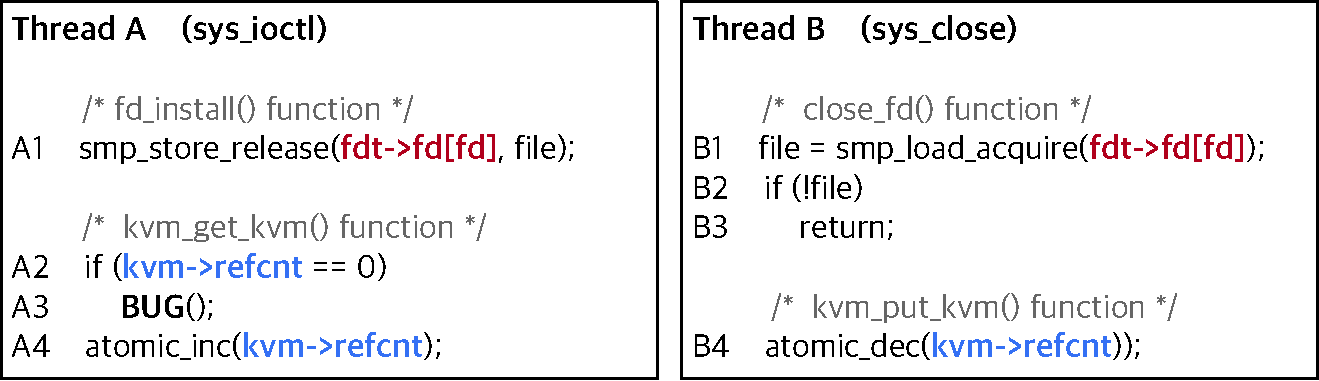
\includegraphics[width=0.9\linewidth]{fig/cve-2017-10661.pdf}
  \caption{Simplified code snippet of CVE-2017-17712. If \texttt{B1}
    is executed between \texttt{A2} and \texttt{A4}, concurrenct
    accesses on \texttt{inet->hdrincl} leads to uninitialized stack
    pointer usage on \texttt{rfv}, and an attacker may gain root
    privileges through a dedicated attack
    technique~\cite{stackspray}.}
  \label{fig:cve-2017-17712}
\end{figure}
%
In \autoref{fig:cve-2017-17712}, an uninitialized access bug may
manifest when two system calls are executed concurrently:
\texttt{sendmsg()} to send a message through an ipv4 socket, and
\texttt{setsockopt()} to modify an option of the ipv4 socket.

Let us assume \texttt{inet->hdrincl} is initially \texttt{1}.
%
During sending a message through the ipv4 socket, thread~A reads a
value of \texttt{inet->hdrincl} twice at \texttt{A2} and \texttt{A4}.
%
However, since these two read operations are not atomically executed,
thread~B may intervene in the middle of these two read operations.
%
In that case, if \texttt{B1} is executed between \texttt{A2} and
\texttt{A4}, thread~A reads different values of \texttt{inet->hdrincl}
at \texttt{A2} and \texttt{A4}, and dereference \texttt{rfv} without
initializing it.


\PP{Observation 1: Combined interleaving orders}
%
This example demonstrates that a concurrency bug is caused by \textit{a combined
  result of multiple interleaving orders}, where each interleaving order
denotes the execution order between an instruction pair that access
the same memory object.
%
In the example of \autoref{fig:cve-2017-17712}, two interleaving orders
are combined to eventually cause the uninitialized access bug.
%
First, \texttt{A2} should be executed before \texttt{B1} (\ie,
$\texttt{A2} \Rightarrow \texttt{B1}$\footnote{In this paper,
  $\texttt{X} \Rightarrow \texttt{Y}$ denotes that \texttt{X} is
  executed before \texttt{Y}}) to make thread~A not initialize
\texttt{rfv}.
%
Second, \texttt{B1} should be executed before \texttt{A4} (\ie,
$\texttt{B1} \Rightarrow \texttt{A4}$) to make thread~A dereference
uninitialized \texttt{rfv} while other interleavings do not 
contribute to the bug.
%
%Therefore, thread interleavings satisfying a combination of the two
%interleaving orders (\ie,
%$(\texttt{A2} \Rightarrow \texttt{B1}) \wedge (\texttt{B1} \Rightarrow
%\texttt{A4}))$ cause the uninitialized access bug, while all other
%thread interleavings do not.
Therefore, to trigger kernel concurrency bugs, a fuzzer must 
consider a combination of multiple interleaving orders. e.g.,
$(\texttt{A2} \Rightarrow \texttt{B1}) \wedge (\texttt{B1} \Rightarrow
\texttt{A4}))$ in \autoref{fig:cve-2017-17712}.


\PP{Design goal 1: Informative interleaving coverage}
\yj{Revisit text to get the point across better}
The observation gives an insight of how to define coverage metric 
in a concurrency fuzzer.
To discover the uninitialized access bug, 
interleaving coverage should not be saturated until
$(\texttt{A2} \Rightarrow \texttt{B1}) \wedge (\texttt{B1} \Rightarrow
\texttt{A4})$ is executed.
%
Otherwise, a fuzzer may think that there is no more interesting thread
interleaving in the multi-thread input, and stop searching for new
thread interleavings of the multi-thread input, missing the
uninitialized access bug.


\PP{Observation 2: Feedback from explored executions}
%
An explored execution that did not cause a concurrency bug provides useful feedback 
to guide what interleaving orders should be further explored.

In the example of \autoref{fig:cve-2017-17712}, let us assume 
if a fuzzer executes the two system calls \textit{sequentially} 
such that thread~A executes all instructions followed by the execution of thread~B.
%
Then, let us also assume that a fuzzer observes the three
instructions, \texttt{A2}, \texttt{A4}, and \texttt{B1}, are executed
in the order of
$\texttt{A2} \Rightarrow \texttt{A4} \Rightarrow \texttt{B1}$, and
access the same memory object~(\ie, \texttt{inet->hdrincl}).
% \yj{can a fuzzer know they are conflicting instructions?}
%
This execution order does not cause the uninitialized access bug.
%
However, from the explored execution, one can easily imagine a new interleaving of these three
instructions by changing the execution order of \texttt{A4} and
\texttt{B1} (\ie,
$\texttt{A2} \Rightarrow \texttt{B1} \Rightarrow \texttt{A4}$).
%
The \yj{speculative} interleaving is what exactly we are looking for; it
satisfies the combination of interleaving orders
$(\texttt{A2} \Rightarrow \texttt{B1}) \wedge (\texttt{B1} \Rightarrow
\texttt{A4}))$, and, if executed, the interleaving order triggers 
the uninitialized access bug.

\PP{Design goal 2: Coverage-based interleaving search strategy}
The observation gives a direction that how a fuzzer should explore 
the search space using a coverage metric.
If interleaving coverage tracks that
$\texttt{A2} \Rightarrow \texttt{A4} \Rightarrow \texttt{B1}$ is
\textit{explored} before, a fuzzer can utilize interleaving
coverage as feedback to infer \textit{unexplored} thread interleavings (\eg,
$\texttt{A2} \Rightarrow \texttt{B1} \Rightarrow \texttt{A4}$). 
This allows a systematic way to explore the search space rather than 
performing randomized search pervasively used in previous approaches~\cite{ski, krace, pctalgorithm, muzz}.%\yj{cite}

In summary, using the coverage metric expressing combinations of interleaving orders and the coverage-based search strategy, a fuzzer can effectively determine what to execute in future iterations, and quickly discover concurrency bugs
without redundantly executing thread interleavings.

\subsection{Limitation of prior approaches}
\label{ss:existingapproaches}
%
% \begin{table}[t]
%   \centering
%   \resizebox{\linewidth}{!}{
  \begin{tabular}{l l l}
    \toprule
    & \thead{\textbf{Interleaving} \\ \textbf{coverage metric}} & \thead{\textbf{Interleaving} \\ \textbf{search strategy}} \\
    \midrule
    \textbf{Razzer~\cite{razzer}} & -- & Coverage-oblivious \\
    \textbf{Krace~\cite{krace}} & Alias coverage & Coverage-oblivious \\
    % & (single instruction pair) & \\
    \textbf{Conzzer~\cite{conzzer}} & Concurrent call pair & Coverage-based (limited) \\
    % & (single function pair) & (limited)\\
    \textbf{Snowboard~\cite{snowboard}} & -- & Coverage-oblivious \\
    \bottomrule
  \end{tabular}
}

%%% Local Variables:
%%% mode: latex
%%% TeX-master: "../p"
%%% End:

%   \caption{Interleaving coverage metrics and interleaving search
%     strategy of recent concurrency fuzzing. ``--'' indicates that a
%     fuzzer does not adopt a concurrency coverage metric. \dr{TODO:
%       rewording}}
%   \label{table:motivation}
% \end{table}

% \autoref{table:motivation} summarizes interleaving coverage metrics and 
% interleaving search strategies of prior approaches.
%
Even though previous approaches achieve their own successes, we find
that their interleaving coverage metrics and interleaving search
strategies do not satisfy \textbf{Design goal 1} and \textbf{2}.


\PP{Less-informative interleaving coverage}
%
We find that previously proposed interleaving coverage metrics are
less-informative because none of them consider a combination of
interleaving orders.

\begin{figure}[t]
  \centering
  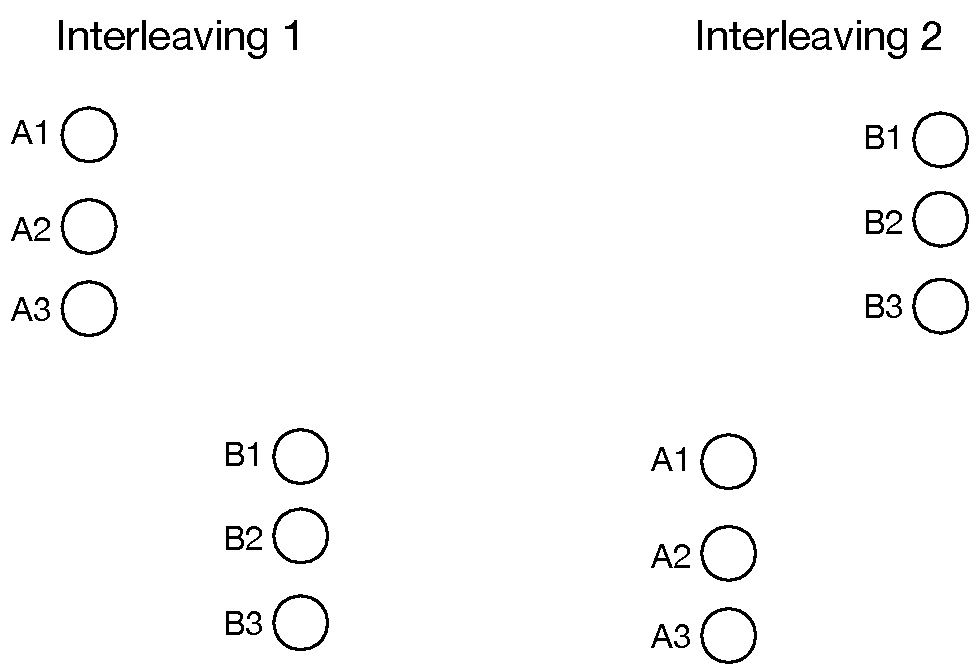
\includegraphics[width=0.8\linewidth]{fig/alias-coverage.pdf}
  \caption{Two thread interleavings between thread~A and thread~B
    described in \autoref{fig:cve-2017-17712}.
    %
    The uninitialized access bug manifests only in
    \texttt{Interleaving \#2}.
    %
    We intentionally omits bug-irrelevant memory accesses (\ie,
    \texttt{A6} and \texttt{B2}).}
  \label{fig:alias-coverage}
\end{figure}



For example, let us suppose we adopt alias coverage~\cite{krace},
which tracks interleaving orders of a \textit{single} instruction
pair.
%
Alias coverage determines a thread interleaving \texttt{X} exposes a
unique behavior if \texttt{X} contains an unexplored interleaving
order $I_W \Rightarrow I_R$, where $I_R$ reads a value written by
$I_W$ and they are executed by different threads.

Then, \autoref{fig:alias-coverage} illustrates the simplified
explanation of why alias coverage does not satisfy the \textbf{Design
  goal 1}.
%
Assuming \texttt{Interleaving \#1} is executed first, alias covereage
identifies \texttt{Interleaving \#1} exposes unique behaviors when it
sees two unexplored interleaving orders (\ie,
($\texttt{B1} \Rightarrow \texttt{A2}$) and
($\texttt{B1} \Rightarrow \texttt{A4}$)).
%
But, when alias coverage faces \texttt{Interleaving \#2} after
\texttt{Interleaving \#1}, it suffers from locating unobserved unique
behaviors of \texttt{Interleaving \#2}, because there is no unobserved
interleaving order in \texttt{Interleaving \#2} (\ie,
($\texttt{B1} \Rightarrow \texttt{A4}$) is already observed in
\texttt{Interleaving \#1}).
%
Therefore, alias coverage may make the wrong decision about whether a
fuzzer needs to run these two system calls more, misleading a fuzzer
to de-prioritize a multi-thread input in which a concurrency bug
resides.


Moreover, concurrent call pair~\cite{conzzer} also suffers from
distinguishing these two thread interleavings.
%
While concurrent call pair tracks a concurrently-executed function
pair, it is not aware of interleavings of instructions.
%
Since two thread interleavings in \autoref{fig:alias-coverage} take
place in the same function (\ie, \texttt{A2} and \texttt{A4} are
executed in the same function), concurrent call pair is also limited
in distinguish the two interleavings, and shows the same limitation as
alias coverage when it comes to discovering this uninitialized access
bug.


% is also saturated with these two thread
% interleavings, because once two functions \texttt{sendmsg()} and
% \texttt{setsockop()} are executed concurrently, concurrnet call pair
% does not matter how a thread interleaving occurs within the function
% pair.





% \yj{This paragraph must be easy enough for reader to intuitively understand, but hard to digest discussions}
% However, they are not applicable to track behavioral changes\yj{what does it mean?} according
% to a combination of interleaving orders, mainly because they either
% track only a \textit{single} interleaving order~\cite{krace, muzz} or
% \textit{coarse-grained information} such as a pair of two
% concurrently-executed functions~\cite{conzzer}.
% \yj{I do not understand why tracking a single int. order and coarse-grain information are not able to track behavioral changes}

% Taking the example of KRace's alias coverage,
% \autoref{fig:alias-coverage} describes two thread interleavings that
% saturate alias coverage found between two system calls in
% \autoref{fig:cve-2017-17712}.
% %
% In these example interleaving scenarios, the uninitialized access does
% not manifest even after alias coverage is saturated, and a fuzzer may
% decide to stop searching for new thread interleavings in the two
% system calls.
% %
% While we do not enumerate all proposed interleaving coverage metrics
% here, we find that they all share the same limitation.


\PP{Coverage-oblivious interleaving search strategy}
%
Stemming from less-informative coverage metrics, proposed interleaving
search strategies are not properly directed by interleaving coverage,
and thus, do not satisfy the \textbf{Design goal 2}.

Since Razzer~\cite{razzer} and Snowboard~\cite{snowboard} do not make
use of interleaving coverage at all, they intrinsically cannot rely on
explored thread interleavings in inferring unexplored thread
interleavings.
%
Krace~\cite{krace} explores thread interleavings randomly without
considering what thread interleavings are explored before. In other
words, Krace utilizes interleaving coverage only when deciding whether
or not to run a multi-thread input more, but not when inferring which
thread interleavings to search in future iterations.
%
Conzzer~\cite{conzzer} is the only work that attempts to direct a
fuzzer based on interleaving coverage, but it's interleaving coverage
metric, concurrent call pair, does not capture interleavings of
instructions, which are true reasons of concurrency bugs.
%
As a consequence, existing approaches do not systematically search for
thread interleavings to run. Rather, they \textit{blindly} go through
trial and error, making redundant executions without exploring
meaningful thread interleavings.






% %
% However, its interleaving coverage (\ie, concurrent call pair) tracks
% thread interleavings in the function-level granularity, and is limited
% in distinguishing tested interleavings and untested interleavings in
% the instruction-level granularity.
% %
% In other words, the Conzzer's interleaving search strategy can direct
% a fuzzer to execute two functions \texttt{raw_sendmsg()} and
% \texttt{do_ip_setsockopt()} concurrently.
% %
% But even after that, Conzzer suffers from triggering the uninitialized
% bug since it is not aware of the execution order of instructions.




% \dr{TODO: MUZZ}


%%% Local Variables:
%%% mode: latex
%%% TeX-master: "p"
%%% End:
